% ref: http://web.mit.edu/8.13/www/revtex4-command-summary.pdf
% sauce: https://hoffman.physics.harvard.edu/example-paper/
\documentclass[
12pt,
tightenlines,
aps,
prb,
twocolumn,
superscriptaddress,
longbibliography,
floatfix
]{revtex4-2}

\usepackage{amsmath,amssymb} % math symbols
\usepackage{bm} % bold math font
\usepackage{graphicx} % for figures
\graphicspath{ {./images/} }
\usepackage{comment} % allows block comments
%\usepackage{ulem} % allows strikeout text, e.g. \sout{text}

\usepackage{minted} % allows colored code
\usepackage{textcomp} % This package gives the text quote '

\usepackage{enumitem}
\setlist{noitemsep,leftmargin=*,topsep=0pt,parsep=0pt}

\usepackage{xcolor} % \textcolor{red}{text} will be red for notes
\definecolor{lightgray}{gray}{0.6}
\definecolor{medgray}{gray}{0.4}




\usepackage{hyperref}
\hypersetup{
colorlinks=true,
urlcolor= blue,
citecolor=blue,
linkcolor= blue,
% bookmarks=true,
% bookmarksopen=false,
}

% Code to add paragraph numbers and titles
\newif\ifptitle
\newif\ifpnumber
\newcounter{para}
\newcommand\ptitle[1]{\par\refstepcounter{para}
{\ifpnumber{\noindent\textcolor{lightgray}{\textbf{\thepara}}\indent}\fi}
{\ifptitle{\textbf{[{#1}]}}\fi}}
\ptitletrue  % comment this line to hide paragraph titles
% \pnumbertrue  % comment this line to hide paragraph numbers

% minimum font size for figures
\newcommand{\minfont}{6}

% Uncomment this line if you prefer your vectors to appear as bold letters.
% By default they will appear with arrows over them.
% \renewcommand{\vec}[1]{\bm{#1}}

% Allows to rewrite the same title in the supplement
\newcommand{\mytitle}{\Huge Face Unlock}

\begin{document}

\title{\mytitle}

\author{
Muhammed Abdullah Shaikh, Khurshed Fitter, Shital Chiddarwar\\
abd@students.vnit.ac.in, khurshedpf@gmail.com, shitalsc@mec.vnit.ac.in\\
\textit{Visvesvaraya National Institute of Technology, Nagpur, India}
}

% \date{}

\begin{abstract}
This is our project report that aims to understand and develop a face recognition framework. We used MNIST, AT\&T and Labelled Faces in the Wild (LFW) datasets during this project. We performed experiment tracking, hyperparameter tuning, and sweeps throughout our work using WandB.\\ Source files are available at: \url{https://github.com/ABD-01/Face-Unlock}.
\end{abstract}

\maketitle

\section{\label{sec:Start}Problem and Motivation}
% \ptitle{Start writing while you experiment} 
% \vspace{-4mm}
Face Recognition is a computer vision task that has been extensively studied for several decades. This project was developed at IvLabs, the AI and Robotics Lab of VNIT, Nagpur. The motivation was to learn and understand the working of face recognition algorithms and \textit{one-shot} learning. Next, we decided to develop the framework for ourselves from scratch and further deploy it on hardware for a face-recognition-based door-lock system.
% \vspace{-5mm}

\section{\label{sec:oneshot}One-Shot Learning}
% \vspace{-4mm}
One-shot learning is a classification task where one example (or a very small number of examples) is given for each class, which is used to prepare a model, that in turn must make predictions about many unknown examples in the future.

This characterizes tasks seen in the field of face recognition, such as face identification and face verification, where people must be classified correctly with different facial expressions, lighting conditions, accessories, and hairstyles given one or a few template photos.

Modern face recognition systems approach the problem of one-shot learning via face recognition by learning a rich low-dimensional feature representation, called face embedding, that can be calculated for faces easily and compared for verification and identification tasks.

Historically, embeddings were learned for one-shot learning problems using a Siamese network. The training of Siamese networks with comparative loss functions resulted in better performance, later leading to the triplet loss function used in the FaceNet system by Google that achieved then state-of-the-art results on benchmark face recognition tasks.
\vspace{-5mm}

\section{\label{sec:Model}Model Architechture}
% \vspace{-4mm}
\ptitle{ResNet} We use residual neural networks for this work, mostly ResNet18, but also experimented with ResNet26 and ResNet50. With ResNets, the gradients can flow directly through the skip connections backward from later layers to initial filters.
% insert residual figure

\ptitle{Siamese Network} A Siamese Neural Network is a class of neural network architectures that contain two or more identical subnetworks. ‘identical’ here means, they have the same configuration with the same parameters and weights. Parameter updating is mirrored across both sub-networks. It is used to find the similarity of the inputs by comparing their feature vectors, so these networks are used in many applications.

\ptitle{Triplet Loss} Triplet loss was introduced in “FaceNet: A Unified Embedding for Face Recognition and Clustering.”
The loss function penalizes the model such that the distance between the matching examples is reduced and the distance between the non-matching examples is increased. Let $d(x,y) : \mathbb{R}^D \times \mathbb{R}^D \rightarrow \mathbb{R}$ be a distance function in embedding space of dimension $D$. The loss function is defined as:
\begin{equation}
L = \sum_{\substack{a,p,n \\ y_a = y_p \neq y_n}} [d(x_a, x_p) - d(x_a, x_n) + \alpha]_+
\label{eqn:tripletloss}
\end{equation}
 This loss makes sure that, projection of an anchor point $x_a$, and it's corresponding positive point $x_p$ belonging to the same class (person) $y_a$ is closer than the projection of a negative point $x_n$ belonging to another class $y_n$, by at least a margin $\alpha$.

\begin{figure}[h]
    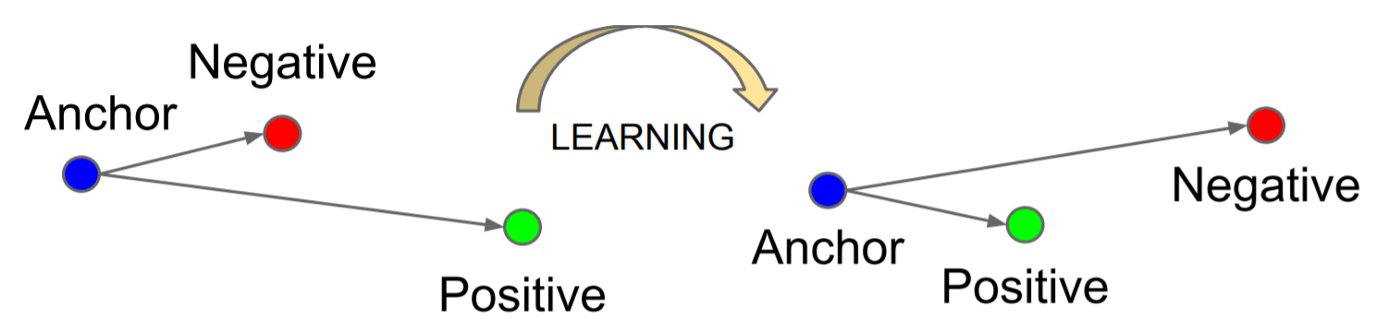
\includegraphics[clip=true,width=\columnwidth]{Tripletloss.png}
    \caption{Triplet Loss} 
     \label{fig:tripletloss}
\end{figure}


% \vspace{-7mm}
\section{\label{sec:Experiments}Experiments}
% \vspace{-5mm}
\subsection{MNIST}
% \vspace{-5mm}
Implemented as a warmup for the project to gain an understanding of one-shot learning and siamese nets.
The model was trained only on 100 images of classes 0,1,2. Images of rest classes i.e 3-9 were kept hidden during the training phase.
The evaluation was done on a 10-way 1-shot basis, wherein the support set \ref{fig:support} had only one sample from each class 0 to 9.

\begin{figure}[h]
    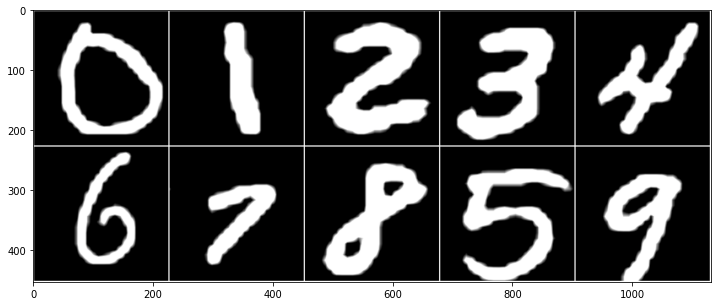
\includegraphics[clip=true,width=\columnwidth]{support.png}
    \caption{Support Set for MNIST one-shot task.} 
     \label{fig:support}
\end{figure}

\onecolumngrid
\begin{center}
\begin{table}[h]
    \centering
    \begin{center}
    \caption{Result on MNIST Dataset}
    \label{tab:mnsit}
    \begin{tabular}{l|cccccccccc}
    \hline
    \textbf{Class}    & 0       & 1       & 2       & 3       & 4       & 5       & 6       & 7       & 8       & 9       \\
    \hline \hline
    \textbf{Correct}  & 5804    & 6648    & 5830    & 5877    & 5830    & 5274    & 5908    & 5589    & 5777    & 5849    \\
    \textbf{Total}    & 5923    & 6742    & 5958    & 6131    & 5842    & 5421    & 5918    & 6265    & 5851    & 5949    \\
    \textbf{Accuracy} & 97.99\% & 98.60\% & 97.85\% & 95.85\% & 99.79\% & 97.28\% & 99.83\% & 89.20\% & 98.73\% & 98.31\%\\
    \hline
    \end{tabular}
    \end{center}
\end{table}
\end{center}
\twocolumngrid

% \vspace{-12mm}
\subsection{AT\&T Face Dataset}
% \vspace{-5mm}
\subsubsection{Dataset Information}
% \vspace{-5mm}
The AT\&T face dataset, “(formerly ‘The ORL Database of Faces’), contains a set of face images taken between April 1992 and April 1994 at AT&T Laboratories Cambridge. It contains 10 different images of 40 distinct people with 400 face images. The database was used in the context of a face recognition project carried out in collaboration with the Speech, Vision and Robotics Group of the Cambridge University Engineering Department.

Besides the fact that the images have the same background and same size, the images were converted to gray level and pixel values were scaled from 0 to 1.
\vspace{-5mm}

\subsubsection{Offline Triplet Mining}
\vspace{-5mm}
In this approach, we first generate the triplets manually and then fit the data to the network. We used two different types of methods
\begin{raggedright}
\begin{enumerate}
    \item All possible triplets - For each image in the dataset (anchor), we choose all possible combinations to make a positive pair, and for each pair choose all possible combination from the remaining class as Negative.
    \item Random triplets - For each image in data (Anchor), randomly sample a Positive image from its class.  Then from each of the other classes sample one image (randomly) as the Negative. Hence, for every Anchor you will have 1 randomly selected positive from it's class and randomly selected Negative from each of the n-1 classes where n is total number of classes.  For every anchor image you would have n-1 triplets. So if you're having 3 classes of 10 images each then you would have 60 triplets
\end{enumerate}
\end{raggedright}
 However this method being too expensive in terms of memory and computation, it was not performed on datasets other than MNIST.

% \vspace{-10mm}
\subsubsection{Online Triplet Mining} 
% \vspace{-5mm}
In this approach, we feed a batch of training data, generate triplets using all examples in the batch and calculate the loss on it. This approach allows us to randomize the triplets and increase the chance to find triplets with high losses. This will help train the model faster.
\begin{figure}[h!]
    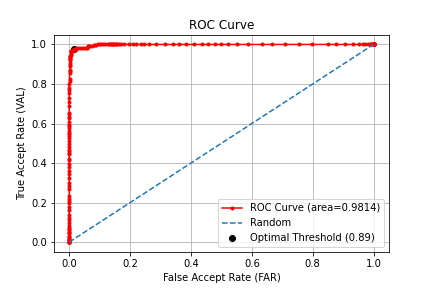
\includegraphics[clip=true,width=\columnwidth]{ROC_curve_ATT_test_dataset.png}
    \caption{An ROC curve is a graph showing the performance of a classification model at all classification thresholds. This curve plots two parameters: (i) True Acceptance Rate, (ii) False Acceptance Rate. The area under ROC curve (AUC) provides an aggregate measure of performance across all possible classification thresholds. AUC = $0.981$} 
     \label{fig:eer_roc}
\end{figure}

\begin{table*}[t]
    \begin{center}
    \caption{Result AT\&T Dataset. $^\dagger$ represents results using online triplet mining, while the rest are using offline mining.}
    \label{tab:att}
    \begin{tabular}{l|c|c|c|c|c}
    \hline
    \textbf{Architechture} & \textbf{No. of learnable parameters} & \textbf{Epochs} & \textbf{Learning Rate} & \textbf{Train Accuracy} & \textbf{Test Accuracy} \\
    \hline \hline
    Plain CNN     & 4,170,400                   & 16     & $0.001$         & 92.67\%        & 88.00\%       \\
    ResNet-18     & 11,235,904                  & 8      & $0.002$         & 99.62\%        & 94.73\%       \\
    ResNet-26     & 17,728,064                  & 20     & $0.002$         & 93.00\%        & 69.00\%       \\
    {ResNet-18}$^\dagger$     & 11,235,904                  & 200    & $0.0002$          & 100\%          & 98.4\%   \\
    \hline
    \end{tabular}
    \end{center}
\end{table*}

% \vspace{100mm}
\subsubsection{Results}
% \vspace{-5mm}
During this experiment, the batch size is 100, the face embedding dimension is 64 and the optimizer used was Adam. The results on this dataset are shown in Table \ref{tab:att}. We also studied the Regional Optical Characteristics (ROC) \ref{fig:eer_roc} and Equal Error Rate (EER) \ref{fig:eer_att} curves for this setting. We further plotted t-SNE chart of the face embeddings to see the clustering behavior of the model shown in \ref{fig:tsne_att}.

\onecolumngrid
\begin{center}    
\begin{figure*}[t!]
    \begin{minipage}[b]{0.45\linewidth}
    \centering
    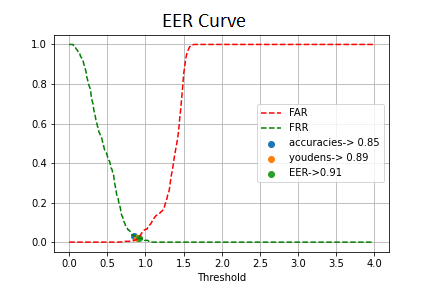
\includegraphics[clip=true,width=1.1\textwidth, height=6cm]{EER_ATT_testdataset.png}
    \caption{The EER is the location on a ROC curve where the false acceptance rate (FAR) and false rejection rate (FRR) are equal. In general, the lower the equal error rate value, the higher the accuracy of the biometric system.}
     \label{fig:eer_att}
     \end{minipage}
     \hspace{0.5cm}
    \begin{minipage}[b]{0.45\linewidth}
    \centering
    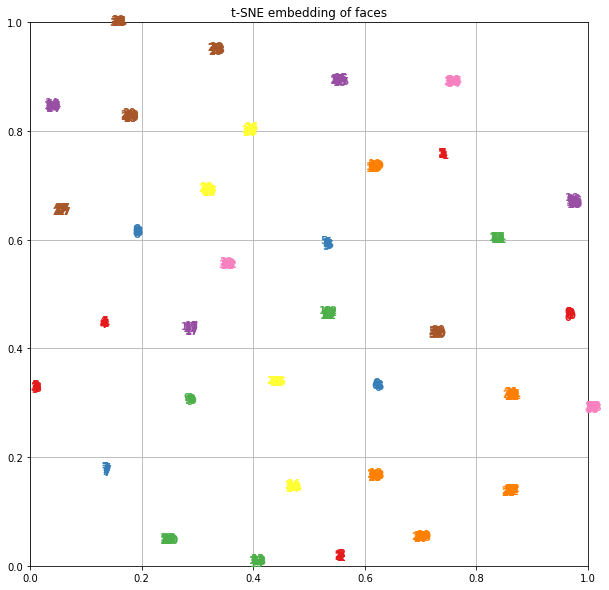
\includegraphics[clip=true,width=\textwidth]{tSNE_embds_ATT_train.png}
    \caption{t-SNE plot for AT\&T dataset.}
    \label{fig:tsne_att}
    \end{minipage}
\end{figure*}
\end{center}
\twocolumngrid

% \vspace{-5mm}
\subsection{Labelled Faces in the Wild (LFW)}
% \vspace{-5mm}
\subsubsection{Dataset Information} 
% \vspace{-5mm}

Labeled Faces in the Wild is a public benchmark for face verification, also known as pair matching. The data set contains more than 13,000 images of faces collected from the web. Each face has been labeled with the name of the person pictured. 1680 of the people pictured have two or more distinct photos in the data set. The only constraint on these faces is that they were detected by the Viola-Jones face detector. 

% \vspace{-5mm}
\subsubsection{Hyperparameter Sweeps}
% \vspace{-5mm}
Hyperparameter search — or tuning, or optimization — is the task of finding the best hyperparameters for a learning algorithm.
Hyperparameter sweeps, enable finding the best possible combinations of hyperparameter values for a specific setting by orchestrating a Run and managing experiments for the configuration of our training.  code. We performed a thorough random search for these hyperparameters using WandB.

\begin{table}[h!]
    \begin{center}
    \caption{Search on model hyperparameters}
    \label{tab:sweep}
    \begin{tabular}{l|c|c}
    \hline
    \textbf{Hyperparameter}                                        & \textbf{\begin{tabular}[c]{@{}l@{}}Range of\\  Search\end{tabular}} & \textbf{\begin{tabular}[c]{@{}l@{}}Selected \\ Value\end{tabular}} \\
    \hline \hline
    Batch Size                                                     & 40,100                                                     & 256                                                       \\
    Epochs                                                         & 10,50,100,200                                              & 200                                                       \\
    \begin{tabular}[c]{@{}l@{}}Learning\\ Rate\end{tabular}        & 0.002, 0.001, 0.0002, 0.0001                               & 0.002                                                     \\
    \begin{tabular}[c]{@{}l@{}}Embedding \\ Dimension\end{tabular} & 64, 128, 256                                               & 128  \\
    \hline
    \end{tabular}
    \end{center}
\end{table}

\begin{figure*}[t]
    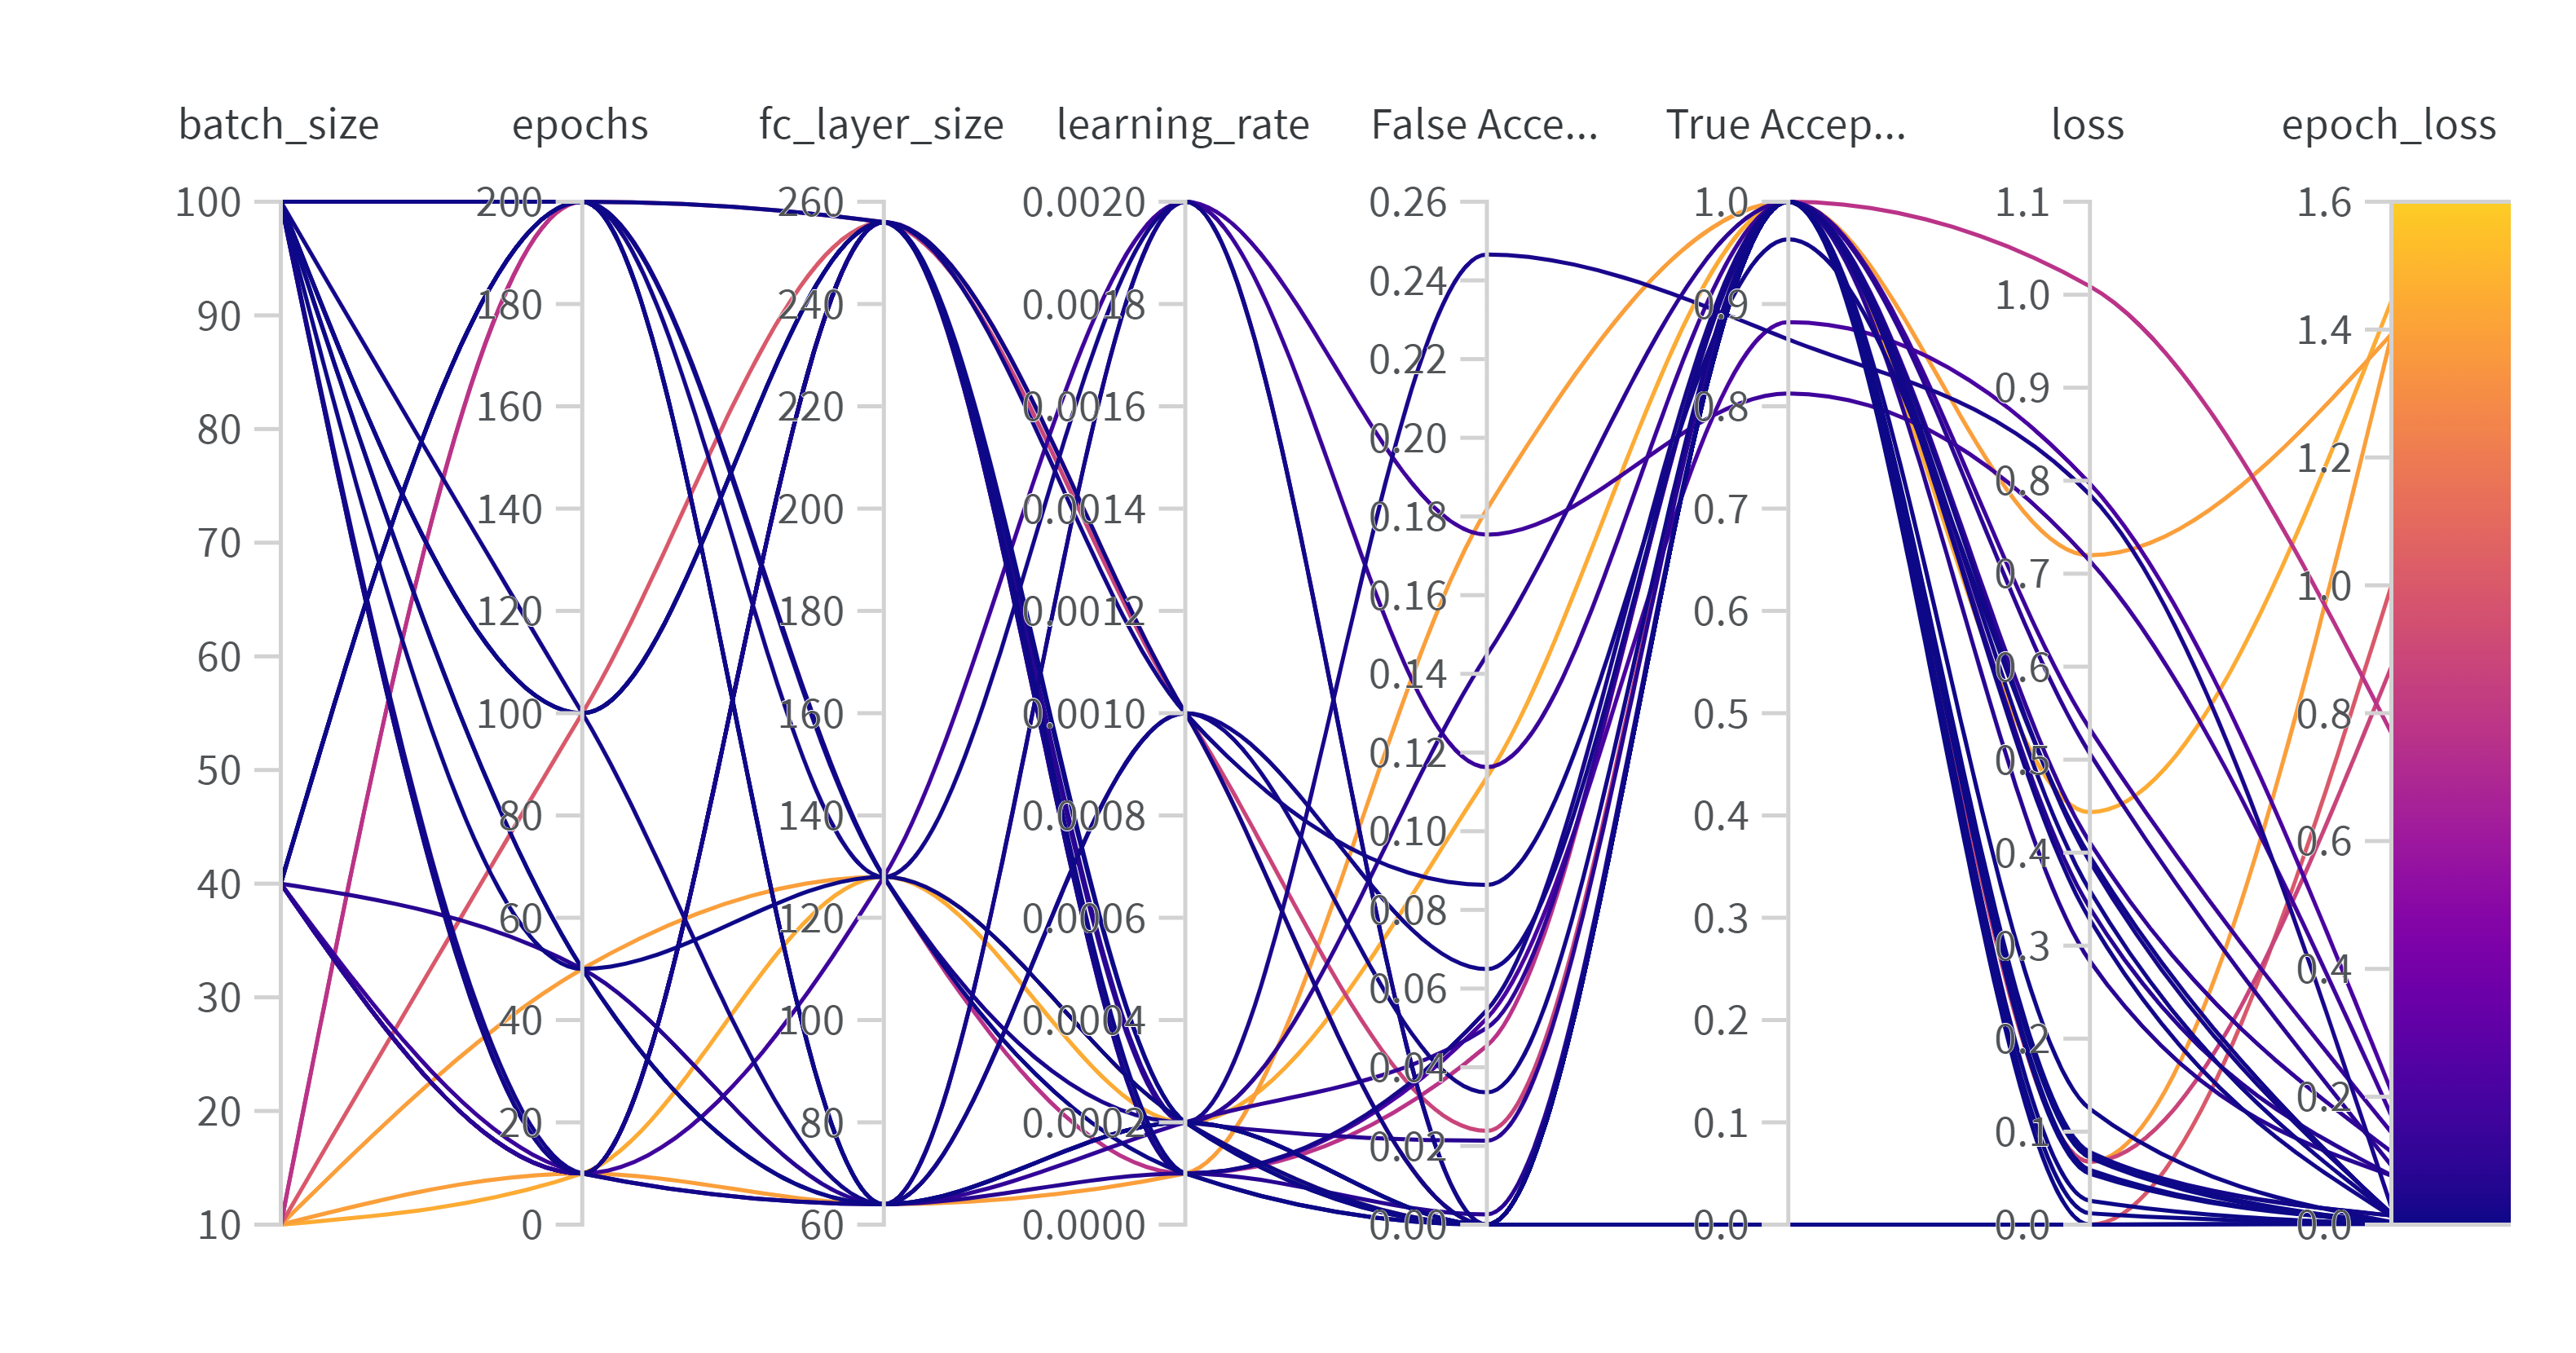
\includegraphics[clip=true,width=2\columnwidth]{face_unlock sweep.png}
    \caption{Hyperparameter Sweep using WandB} 
     \label{fig:sweep}
\end{figure*}

% \vspace{-5mm}
\subsubsection{Results}
% \vspace{-5mm}
We use the ResNet-18 architecture and the weights provided by He et al. [14]. We discard the last layer and add a fully connected layer of size 128 corresponding to the embedding dimension. The optimizer used was Adam with a weight decay of 0.01 and rest hyperparameters as mentioned in \ref{tab:sweep}. We start with a learning
rate of $2\times10^{-3}$, and divide it by 2 at every 50 epochs, the chance in learning rate is depicted in \ref{fig:lr}. We train with batch hard triplet loss as shown in In Defense of the Triplet Loss for Person Re-Identification. We evaluate our performance on benchmark for comparison, 10-fold cross validation split provided on the official website of LFW. Apart from accuracy, we also studied TAR, FAR and precision of the model. 

\ptitle{Biometrics} There are four possible outcomes from a binary classifier. If the outcome from a prediction is \textit{p} and the actual value is also \textit{p}, then it is called a \textit{true positive} (TP); however if the actual value is \textit{n} then it is said to be a \textit{false positive} (FP). Conversely, a \textit{true negative} (TN) has occurred when both the prediction outcome and the actual value are \textit{n}, and \textit{false negative} (FN) is when the prediction outcome is \textit{n} while the actual value is \textit{p}. The performance of biometric systems is expressed on the basis of the following error rates:
\begin{raggedright}
\begin{enumerate}
\item \textit{Accuracy} $\displaystyle{ = \frac{\text{TP + TN}}{\text{TP+FP+FN+TN}}}$
\item \textit{True Acceptance Rate} also known as \textit{sensitivity} or \textit{recall}
\begin{equation}
\nonumber \displaystyle{\text{TAR} = \frac{\text{TP}}{\text{TP+TN}} = 1-\text{FRR}}
\end{equation}
\item \textit{False Acceptance Rate (FAR)}
\begin{equation}
\nonumber \displaystyle{\text{FAR} = \frac{\text{FP}}{\text{FP+TN}} = 1-\text{TAR}}
\end{equation}
\item \textit{True Rejection Rate (TRR)} also known as \textit{specificity}
\item \textit{False Rejection Rate (FRR)}
\end{enumerate}
\end{raggedright}
The ROC curve \ref{fig:roclfw} is useful to understand the trade-off in TAR and FAR for different thresholds. We use Youden’s J statistic to determine the best threshold for the classification. 
\begin{eqnarray}
\nonumber {\displaystyle J={\text{sensitivity}}+{\text{specificity}}-1} \\
\nonumber {\displaystyle J={\frac {\text{TP}}{{\text{TP}}+{\text{FN}}}}+{\frac {\text{TN}}{{\text{TN}}+{\text{FP}}}}-1}
\end{eqnarray}

% \begin{figure*}[!b]
%     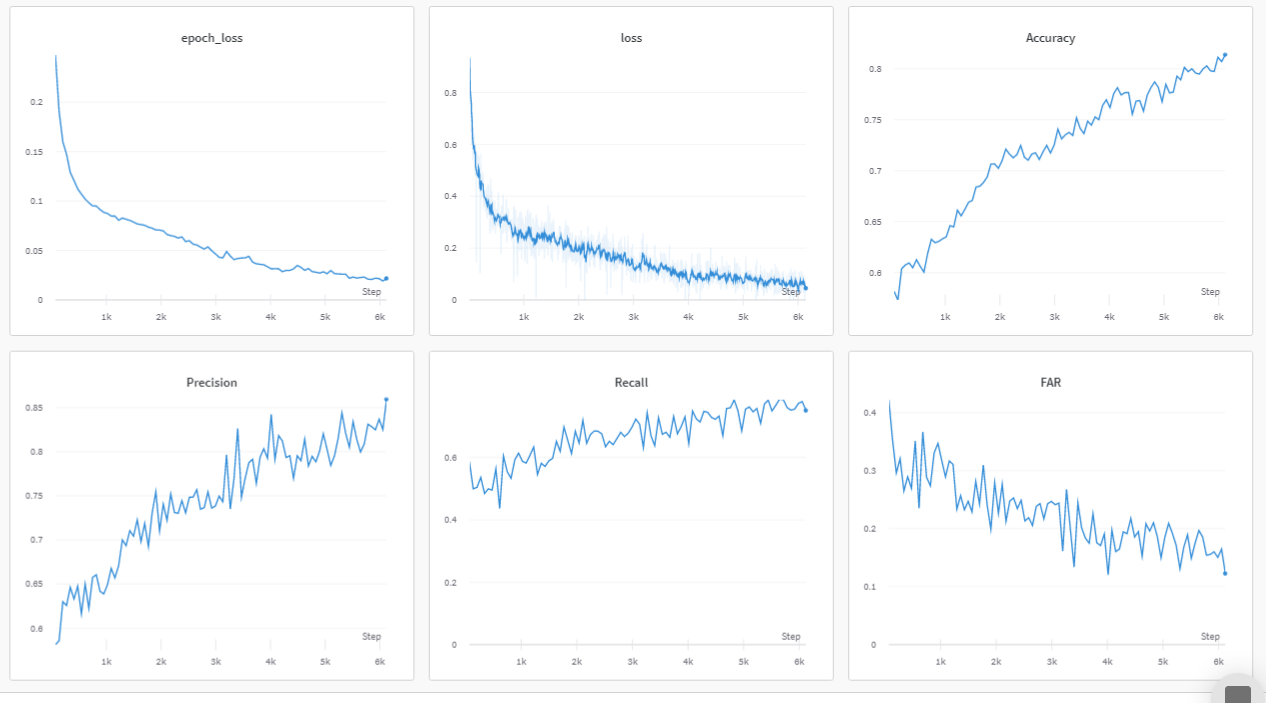
\includegraphics[clip=true,width=2\columnwidth]{wandb.png}
%     \caption{Training Curves} 
% \end{figure*}

\begin{figure}[h]
    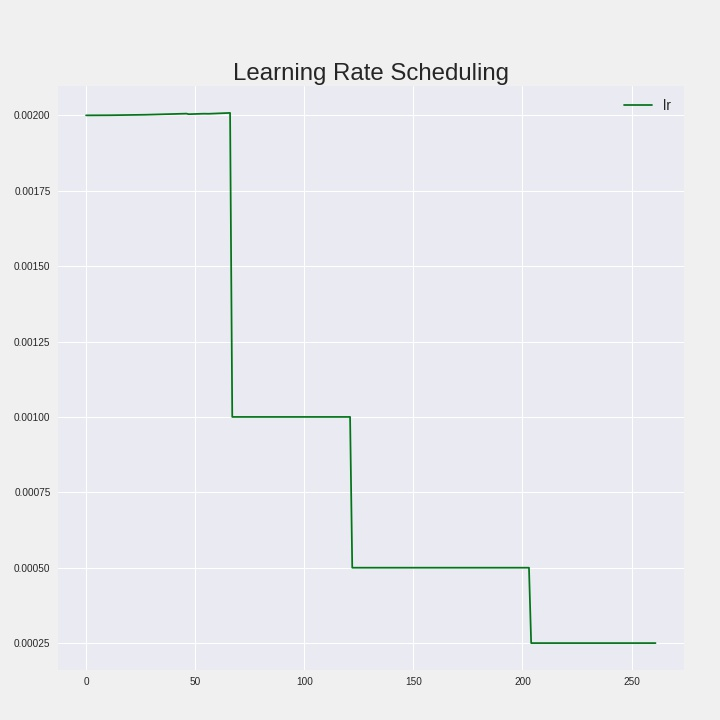
\includegraphics[clip=true,width=\columnwidth, height=\columnwidth]{LFWfinal_lr.jpeg}
    \caption{Learning Rate} 
     \label{fig:lr}
\end{figure}


\begin{figure*}[h!]
    \begin{minipage}[b]{0.45\linewidth}
    \centering
    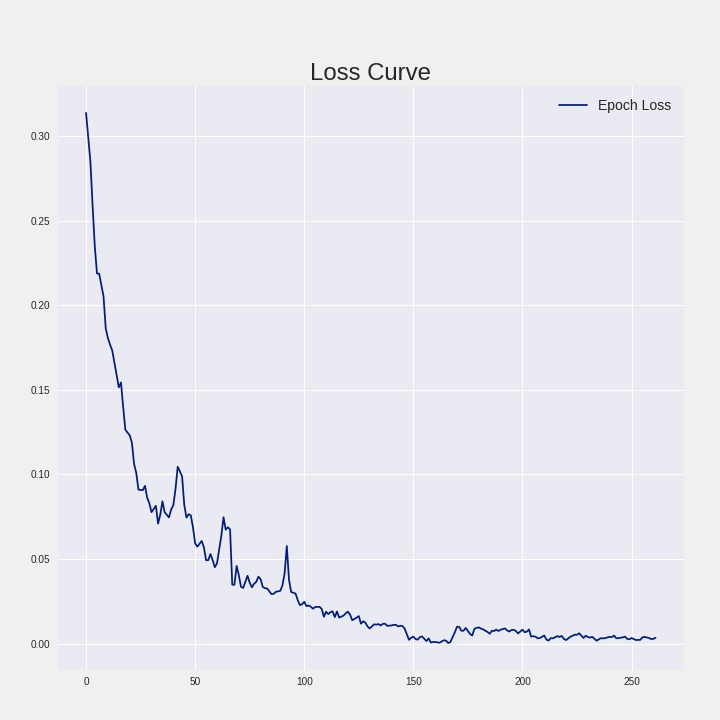
\includegraphics[clip=true,width=1.1\textwidth, height=8cm]{LFWfinal_epochloss.jpeg}
    \caption{Epoch Loss}
     \label{fig:epoch_loss}
     \end{minipage}
     \hspace{1cm}
    \begin{minipage}[b]{0.45\linewidth}
    \centering
    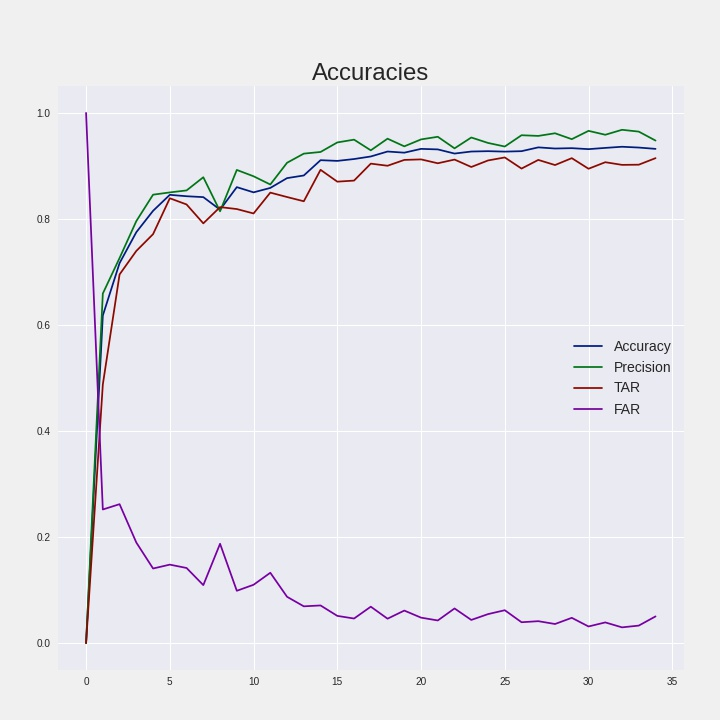
\includegraphics[clip=true,width=\textwidth, height=8cm]{LFWfinal_acc.jpeg}
    \caption{Learning Curves}
    \label{fig:acc}
    \end{minipage}
\end{figure*}

\begin{figure}[h]
    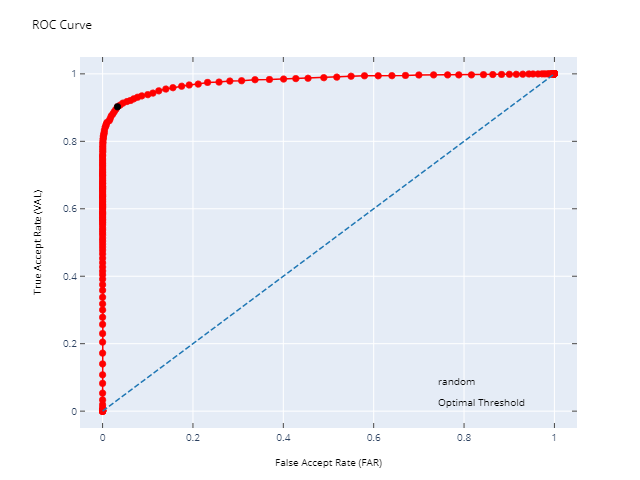
\includegraphics[clip=true,width=\columnwidth]{roc.png}
    \caption{ROC Curve. The Optimal threshold is found to be $1.10$ at TAR=0.864, FAR=0.133. TAR$@$FAR=0.01 is found to be $0.5963$} 
     \label{fig:roclfw}
\end{figure}


% \section{\label{sec:References}References}

% \noindent Referencing should be done using BibTeX.
% \begin{itemize}[label=$\Box$]

% \item Consistently use reference tags that will be easily recognizable and editable from the tex file, e.g. {\tt AuthorJournalYear}. Suppose you will be citing
% Huang {\it et al}, Nano.\ Lett.\ 16, 4224 (2016) \cite{HuangNanoLett2016} and
% Huang {\it et al}, Phys.\ Rev.\ B 93, 125129 (2016) \cite{HuangPRB2016}.
% Instead of {\tt Huang2016a} and {\tt Huang2016b}, use {\tt HuangNanoLett2016} and {\tt HuangPRB2016}. (Note: You can make these bib tags within Mendeley.)

% \item Spend 5 minutes to use find-replace with regular expressions to delete the abstracts, keywords, and other useless information from your bib file, to make it easier to read.
% \item Alphabetize the bib entries by author last name, so that it will be easy to notice if there are duplicates. (Note: Mendeley can automatically export them in alphabetical order.)
% \item The hyperlink should be generated from the doi, so make sure every bib entry has a valid doi. You should delete the URL field (unless you are specifically citing a website), because it may contain a non-general URL such as \url{https://journals-aps-org.ezp-prod1.hul.harvard.edu/prb/abstract/10.1103/PhysRevB.93.125129}.
% \item Check the \LaTeX\ formatting of any special characters in the author's names, e.g. {\tt S\textbackslash\textquotesingle\{a\}nchez}
% \item Check the \LaTeX\ formatting in the titles. You need to use extra \{\} around any letters that should be capitalized, e.g.\ {\tt title = \{Quantum Anomalous \{H\}all Effect\} }
% \item Chemical formulas should also be enclosed in \{\} so element abbreviations will be capitalized, e.g.\ {\tt title = \{Experiments on \{Bi\$\_2\$Se\$\_3\$\}\}}. Don't use excessively complicated formatting for chemicals. Just put the subscripts in \$\$.
% \item Use {\tt longbibliography} in the documentclass at the top of the tex file, so that the title of each paper appears in the references.
% \item For most citations, you can just use {\tt \textbackslash cite\{AuthorJournalYear\}}, e.g.\ Jeehoon used conducting force microscopy to measure a metal-insulator transition \cite{KimAPL2010}. But if you're using a superscript citation style, and the citation comes directly after a number or chemical formula, use {\tt Ref.\textbackslash\ \textbackslash onlinecite\{AuthorJournalYear\}} instead to avoid confusion, e.g.\ Jessie measured the pinning force on vortices in NdFeAsO$_{1-x}$F$_x$ (Ref.\ \onlinecite{ZhangPRB2015}).
% \item In the compiled PDF, check all the references carefully to make sure they have correctly formatted authors, titles, and hyperlinks.
% \end{itemize}

% \section{\label{sec:Integrity}Professional Integrity Checklist}

% \begin{itemize}[label=$\Box$]
% \item Authorship -- are all major contributors and collaborators included? See the American Physical Society guidelines for authorship \cite{APSauthor}.

% \item Plagiarism -- have you been careful to distinguish between your own work and ideas, as opposed to those of others?

% \item Citations -- have you properly cited prior work, and references that you used?

% \item Data Integrity -- have you clearly described the data analysis methods, and justified any data points that were excluded?

% \item Image Processing -- have you clearly described any processing that was applied to images?

% \item Acknowledgments -- have you given appropriate credit and thanks to collaborators and other individuals or organizations who deserve recognition?

% \item Clarity of collaborative structure -- if this is a joint effort, have you identified people who you worked with on this project? Acknowledgments should clearly state who did which parts of the experiment \& analysis, and who wrote the paper.

% \item Conflicts of Interest -- do you have any conflicts of interest where you or someone close to you stands to gain, financially or otherwise, from this work?
% \end{itemize}

% \section{\label{sec:Conclusion}Final Checklist}

% \begin{itemize}[label=$\Box$]
% \item Think critically about all of your own claims {\em and} about all of the claims made by your coauthors. If you do not understand something that your coauthor has written in the draft, push back until you do understand, then suggest an alternative phrasing to clarify the manuscript or figure.
% \end{itemize}

% \begin{acknowledgments}
% We acknowledge advice from Jessie Zhang and Harry Pirie to produce Fig.\ \ref{fig:pixels}. We also acknowledge a generation of students who have made all of the errors that led to these checklists.
% \end{acknowledgments}

% \appendix

% \section{\label{app:Mendeley}Mendeley}

% Mendeley provides a convenient (although not 100\% bug-free) database structure for storing, sorting, and annotating the papers you read. Mendeley also provides an export function to automatically create your bib file. Here are some tips to use Mendeley most effectively.
% \begin{enumerate}
% \item Download Mendeley: \url{http://www.mendeley.com/}\\ Launch it on your desktop.
% \item Set Mendeley options: Make sure your Mendeley database is set correctly to include the DOI (digital object identifier) field. Go to Tools $\rightarrow$ Options $\rightarrow$ Document Details. Scroll down and make sure the DOI box is checked.
% \item Import paper: In the upper left corner of Mendeley Desktop, click the drop-down menu for ``Add'' and select the bottom option ``Add Entry Manually''. In the dialog box that pops up, scroll down until you find the DOI field. Paste the DOI into the field, and click the little magnifying glass icon to the right of the field. This will auto-populate all of the relevant paper information such as author names, title, etc., without risk of typos due to manual copying.\\
%     \textit{Note 1:} Mendeley also allows you to import directly from a PDF file, and it tries to pull all of the meta-data from the PDF, but the process is imperfect. So it's safest to use the DOI for an error-free import.\\
%     \textit{Note 2:} Even if you use the DOI, some journal titles will not import correctly with special characters, so you may need to manually correct.
% \item Add tags: It's useful to add tags to help sort your imported papers. For example, if you are going to be writing a manuscript in 2019 on superconductivity, you might add the tag ``sc19'' to all the relevant papers that you will be citing in your manuscript.
% \item Export bib file: Select all of the references that you want to include, and go to File $\rightarrow$ Export.  Name your file, and it will add a citation key to each paper (e.g.\ Whitesides2004) and automatically export to a bib file.
% \item Resolve redundant citation keys: At this point, you may have several references with the same citation key, e.g.\ Huang2016a and Huang2016b \cite{HuangNanoLett2016, HuangPRB2016}. For your future convenience, you should manually change the redundant citation keys to be more informative, e.g.\ HuangNanoLett2016 and HuangPRB2016. Now re-export the bib file.
% \item Open the bib file in your tex file editor. By default, Mendeley exports all fields, including long ones like the abstract. To reduce clutter in your bib file, and make it easier to debug any errors, it's a good idea to remove the abstracts and other unnecessary fields. For example, in WinEdt go to Search $\rightarrow$ Replace, check the regular expressions box, search for ``{\tt <abstract**\textbackslash\},>},'' and replace it with nothing.
% \end{enumerate}

% \section{\label{app:REVTeX}REVTeX}

% \noindent How to install REVTeX 4-2 on Windows for MikTex:
% \begin{enumerate}
% \item Download REVTeX 4-2:\\ \url{http://authors.aps.org/revtex4/}
% \item Unzip the downloaded folder revtex4-2-tds
% \item If you don't already have one, create a folder C:\textbackslash TeX-local
% \item Copy the four subfolders (bibtex, doc, source, tex) into C:\textbackslash TeX-local
% \item From the start menu, open MikTex 2.9 $\rightarrow$ Maintenance (Admin) $\rightarrow$ Settings
% \item On the root tab, add the path C:\textbackslash TeX-local
% \item On the general tab, click ``Refresh FNDB''
% (You may need to close WinEdt, or whatever is using your MikTex installation, in order to properly ``Refresh FNDB''.)
% \item Download natbib:\\
% \url{http://www.ctan.org/tex-archive/macros/latex/contrib/natbib/}
% \item Unzip natbib.
% \item Open natbib.ins, and run TeX on it (Shift+Ctrl+T in WinEdt)
% \item Open bibentry.ins, and run TeX on it (Shift+Ctrl+T in WinEdt)
% %\item You may also need to get two more packages, i.e.\ download from ctan and run TeX on url.ins and textcase.ins
% \end{enumerate}

% %\newpage % acts like \columbreak for a 2-column doc
% \section{\label{app:vectorfig}Vector Graphics}

% To create vectorized graphics from python, include {\tt rasterized=True} inside the {\tt imshow} command. Unfortunately, this preference doesn't seem to be allowable as a default in any style sheet, so you need to remember to include it it every time. Then save the python figure as a PDF, which ensures that annotations (like scale bars, axis labels, and lines) remain as vector format, but images retain their proper pixelation. For example:

% \begin{minted}[mathescape, linenos]{python}
% fig, ax = subplots(1, 1, figsize=[1.8,1.6])
% ax.imshow(a.Z, cmap=stmpy.cm.blue2, aspect=1,
%   clim=(0,1.4), rasterized=True)
% ... 
% tight_layout(pad=0)
% savefig("topo.pdf")
% \end{minted}

% \noindent Note that some PDF viewers apply their own smoothing to images. For example, MacOS Preview may blur images that look fine in Adobe Illustrator.

\bibliography{Hoffman-example-paper}

\end{document}
